%   Filename    : chapter_4.tex 


\chapter{Preliminary Results/System Prototype}
This chapter presents the preliminary results between the comparison of trained machine learning models: Logistic Regression, Random Forest,  Decision Trees, Support Vector Machine (SVM), and k-nearest Neighbors (KNN).  This chapter will also present the model evaluation and the comparison of model performance. 

\section{Data Summary}
\subsection{Dataset Overview}

The dataset contains the morphological measurements collected from the 50 male and 50 female T. granosa samples. The morphological characteristics included in the dataset are the length, width, height, rib count, hinge length, and distance between the umbos. Additional ratio-based characteristics, such as Length-to-Width ratio, and Length-to-Height ratio, were computed to take into consideration the size variations. These ratios were calculated by dividing the shell length by the shell width and height, respectively. 

\subsection{Preprocessing Results}

The preprocessing of the data includes data cleaning, feature engineering, and encoding. Any missing data entries were removed throughout the data cleaning process. The LW and LH ratios were calculated and added by feature engineering to standardize size variations among the samples while maintaining significant morphological patterns. Additionally, a categorical label was encoded using binary values. It was done by indicating male as 1 and female as 0. As for the final preparation, the dataset was split into 70\% as the training and 30\% as testing to ensure balanced male and female sample representation in the training set as well as in testing sets.

\section{Hyperparameter Optimization}

Hyperparameter optimization was conducted using Grid Search Cross-Validation (GridSearchCV) to improve the performance and reliability of the machine learning models. This was done systematically by fine-tuning key parameters to find the best combination that maximizes model accuracy, precision, recall, and F1-score (Belcic and Stryker, 2024). Table~\ref{tab:hyperparameter-optimization} shows the summarized resulting parameters and corresponding scores for each model.

\begin{table}[H]
	\centering
	\resizebox{\linewidth}{!}{ 
		\begin{tabular}{lcc}
			\hline
			\textbf{Model} & \textbf{Best Parameters} & \textbf{Score}  \\ \hline
			Logistic Regression & \{'classifier\_\_C': 5\} & 0.744654  \\
			Decision Tree       & \{'criterion': 'gini', 'max\_depth': 10\} & 0.986164  \\
			Random Forest       & \{'n\_estimators': 50\} & 0.991195  \\
			SVM                 & \{'classifier\_\_C': 20, 'classifier\_\_kernel': 'rbf'\} & 0.862893  \\
			KNN                 & \{'classifier\_\_metric': 'manhattan', 'classifier\_\_n\_neighbors': 9, 'classifier\_\_weights': 'distance'\} & 0.991195  \\ \hline
		\end{tabular}
	}
	\caption{Best parameters and accuracy scores for the machine learning models.}
	\label{tab:hyperparameter-optimization}
\end{table}

For Logistic Regression, the best hyperparameter was the regularization strength, C (1, 5, and 10), with the best score being obtained when C=5. The score was 0.7447, which implies a balance between model complexity and overfitting prevention.

The Decision Tree model was optimized by tuning the criterion for splitting (gini and entropy) and the maximum tree depth (5 and 10). The best combination used the Gini impurity criterion and a maximum depth of 10. It resulted in a score of 0.9862. This setup effectively balanced the trade-off between catching data patterns and preventing over-complexity. 

For the Random Forest model, n\_estimators (10, 15, 20, 50, 100, and 200) were tuned. Using 50 estimators gave the best performance with a score of 0.9912 which indicates the strength of the ensemble model in capturing diverse data patterns and reducing variance.

A support vector machine was tuned using regularization parameters (1, 10, and 20) and kernel (rbf and linear) where RBF kernel and a regularization parameter of 20 showed superior performance with a score of 0.8629. This configuration well captures how the model can really handle the non-linear relationship in the dataset. 

The k-Nearest Neighbors (KNN) algorithm was tuned using the number of neighbors (3, 5, 7, and 9), distance metric (euclidean and manhattan), and weighting scheme (uniform and distance), with n\_neighbors of 9, manhattan distance metric, and distanced-based weighting yielding a satisfactory score of 99.1\%.

\section{Tuned Classifier Comparison}

After hyperparameter tuning, the performance of the classifiers was re-evaluated to compare their efficiency and accuracy. The evaluation of the models considered balanced accuracy and training time to know which model is more appropriate for practical use in predicting sex in T. granosa. Table~\ref{tab:tuned-classifier-comparison} shows the balanced accuracy percentages obtained by each tuned classifier along with the corresponding training times.

\begin{table}[H]
	\centering
	\resizebox{\linewidth}{!}{ 
		\begin{tabular}{lcc}
			\hline
			\textbf{Model} & \textbf{Balanced Accuracy (\%)} & \textbf{Training Time (s)}  \\ \hline
			Logistic Regression & 74.35 & 3.07  \\
			Decision Tree       & 95.44 & 0.16  \\
			Random Forest       & 98.73 & 1.29  \\
			SVM                 & 74.64 & 0.12  \\
			KNN                 & 83.05 & 0.15  \\ \hline
		\end{tabular}
	}
	\caption{Balanced accuracy and training time for each machine learning model.}
	\label{tab:tuned-classifier-comparison}
\end{table}

Among the models, Decision Tree had the highest balanced accuracy of 99.44\% and took 0.16 seconds for training. Random Forest showed a balanced accuracy of 98.73\% but took 1.29 seconds for training. The model SVM was also very close with a training time of 0.12 seconds but a much lower balanced accuracy at 74.64\%. In terms of training time, Logistic Regression was the slowest to train at 3.07 seconds and recorded the lowest accuracy at 74.35\%. On the other hand, KNN showed a pretty balanced accuracy of 83.05\% and took only 0.15 seconds to train. However, it wasn't as good as Decision Tree and Random Forest. These results indicate that while the Decision Tree proved to be the most accurate and fastest classifier for the dataset, the Random Forest had comparable accuracy with a slightly longer training time.

Figure~\ref{fig:confusion matrices} shows the confusion matrices that allow for a detailed breakdown of classifier predictions including true positives (correctly identified females), true negatives (correctly identified males), false positives (males incorrectly classified as females), and false negatives (females incorrectly classified as males).

Logistic Regression had achieved 69 true positives and 104 true negatives. However, there were also 22 false positives and 33 false negatives, so it actually has not been optimal and so does not differ as perfectly between male and female samples of T. granosa, agreeing to its low balanced accuracy with 74.35\%. The large number of the wrongly classified data points can only indicate that Logistic Regression suffers from the complexity of this dataset.

The Decision Tree classifier gave perfect results, true positives at 102, and true negatives at 126, without any false positives or negatives. This reflects the ability of the model to capture very fine patterns in the morphological traits, thus having an excellent balanced accuracy of 99.44\%.

Similar to the Decision Tree, Random Forest achieved perfect classification with 102 true positives and 126 true negatives with no false positives or false negatives. The ensemble approach of this model contributed to its robustness, which gave it an excellent balanced accuracy of 98.73\%.

SVM correctly classified 87 samples as true positives and 124 as true negatives but had 2 false positives and 15 false negatives. Although better than Logistic Regression, misclassifications in both indicate difficulties in capturing all the complexities of the dataset completely. It is evident from the fact that its balanced accuracy is also lower at 74.64\%.

KNN was perfect in classification results with 126 true positives and 102 true negatives, and no misclassifications. Its balanced accuracy is 83.05\%, which shows that it has a good ability to work well with local data patterns.

The confusion matrix results show that Decision Tree, Random Forest, and KNN performed great in classifying male and female T. granosa with no mistake. In contrast, Logistic Regression and SVM showed more errors, and their performance underscores the limitations of such models. These results prove that non-parametric methods like KNN and ensemble approaches like Random Forest are suitable for this kind of data set of morphological features.

\begin{figure}[!htbp]
	\centering
	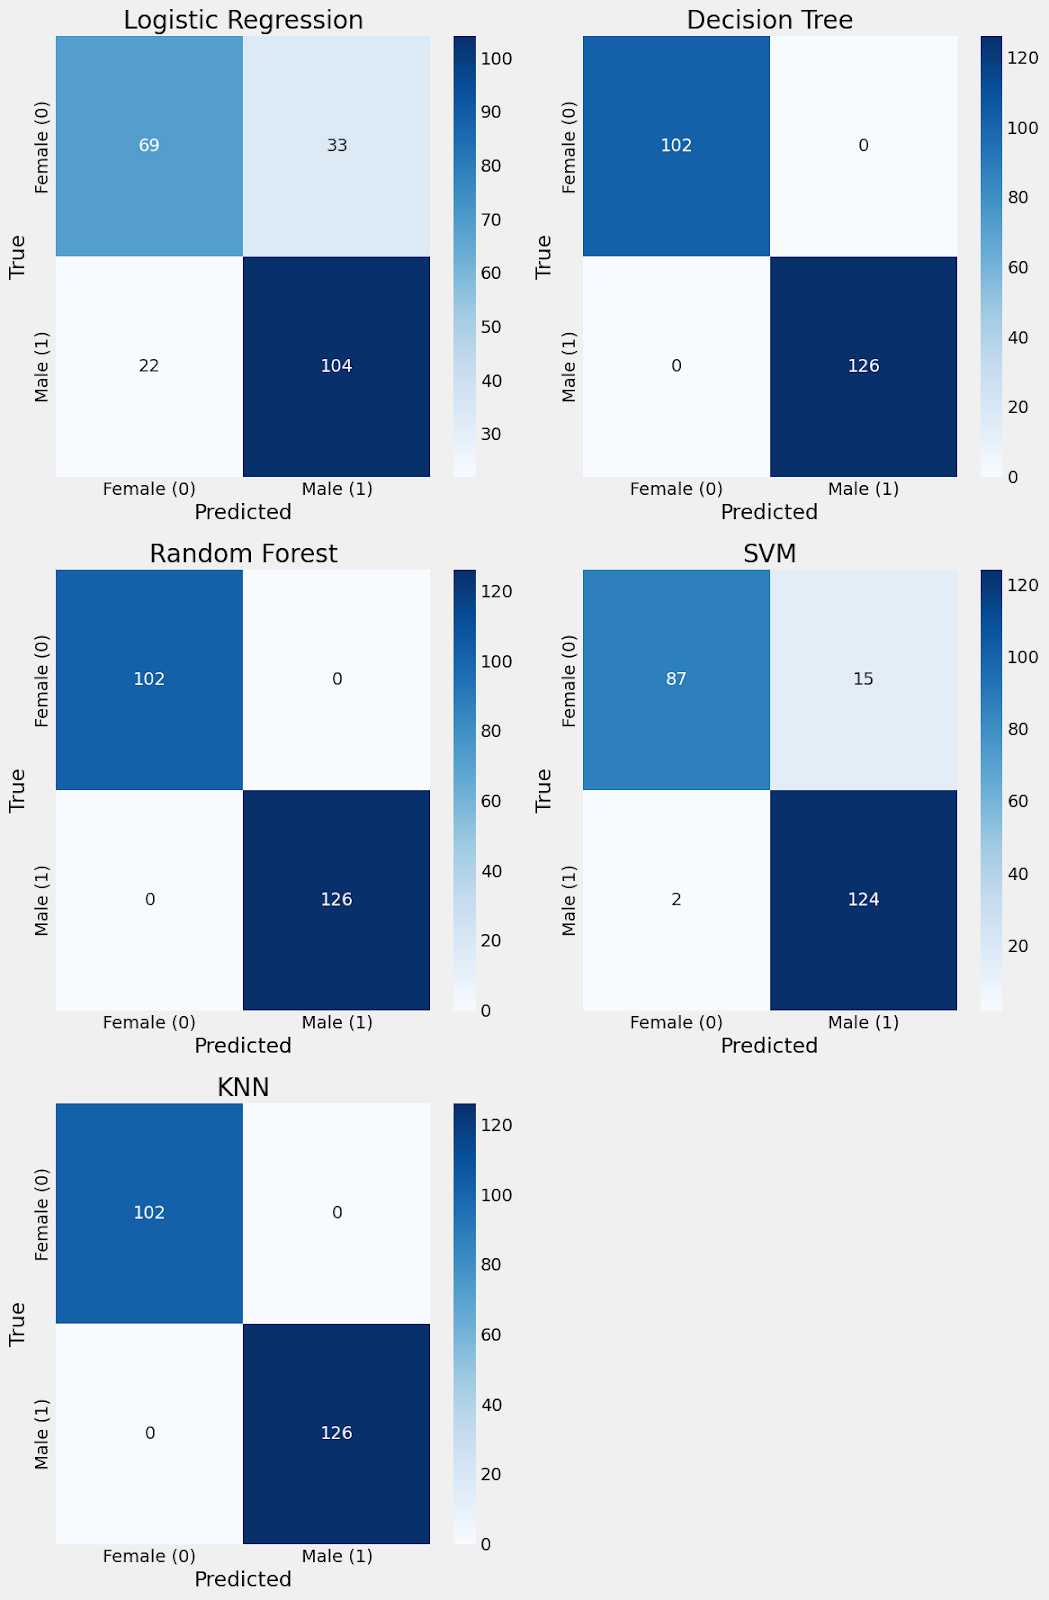
\includegraphics[width=0.95\textwidth]{figures/confusion matrices.png}
	\caption{Confusion Matrices of the Machine Learning Models}
	\label{fig:confusion matrices}
\end{figure}

\section{Comparison of Model Performance}

To evaluate the performance of the different models used, the effectiveness of the models was evaluated and compared in predicting the sex of the \textit{T. granosa} based on morphological traits. The use of performance metrics such as accuracy, precision, recall, and F1-score is used to evaluate the performance of the different models. By analyzing the performance metrics, the researchers can identify the most effective and best model for the classification of male and female \textit{T. granosa}. 


\begin{table}[H]
	\centering
	\resizebox{\linewidth}{!}{ 
		\begin{tabular}{lcccc}
			\hline
			\textbf{Model} & \textbf{Ave Accuracy (\%)} & \textbf{Ave Precision (\%)} & \textbf{Ave Recall (\%)} & \textbf{Ave F1-score (\%)} \\ \hline
			Logistic Regression & 78.86 & 74.96 & 74.86 & 74.55 \\
			Decision Tree       & 98.11 & 98.22 & 98.11 & 98.12 \\
			Random Forest       & 98.68 & 98.74 & 98.68 & 98.68 \\
			SVM                 & 87.34 & 87.79 & 87.34 & 87.22 \\
			KNN                 & 99.43 & 99.45 & 99.43 & 99.43 \\ \hline
		\end{tabular}
	}
	\caption{Model Performance Comparison}
	\label{tab:model-performance}
\end{table}

Table ~\ref{tab:model-performance} presents the comparison results of machine learning models on the morphological traits of the combined  male and female \textit{T. granosa} datasets. The results indicate that all models demonstrated high performance in predicting male and female, with the F1-score ranging between 74-99\%. The KNN model achieved the highest accuracy (99.43\%), precision (99.45\%), recall (99.43\%) and F1-score (99.43\%), followed by random forest, decision tree, and SVM, respectively. However, the logistic regression was the worst classifier having an accuracy of (74.86\%), precision (74.96\%), recall (74.86\%) and (74.55\%) F1-score. Overall, the results seen in this comparison highlight that machine learning models are highly effective in predicting sex identification of \textit{T. granosa} based on their morphological features. With KNN being the best model, it suggests that non-parametric data and pattern recognition (H. Benhar, 2020) is well suited for this dataset. 

\section{Feature Importance Analysis}
After processing the dataset and splitting it into training and testing sets, the models are trained and their important features are computed. Feature analysis helps in identifying which morphological features contribute most in classifying male and female \textit{T. granosa}. The study uses models such as decision trees, and random forests to generate the scores. The models explore a wide range of features and then produce a score that reflects the feature’s importance in predicting the variable (Anitha \& Neelakandan, 2024).  

\begin{figure}[!htbp]
	\centering
	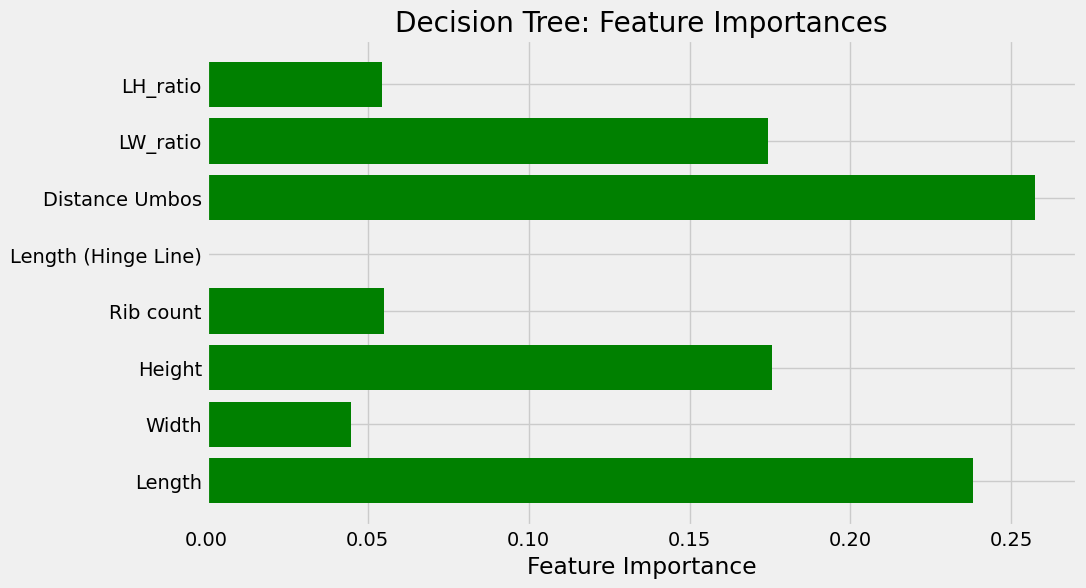
\includegraphics[width=0.8\textwidth]{figures/decision-trees.png}
	\caption{Feature Importance of Decision Trees}
	\label{fig:decision-trees}
\end{figure}

\begin{figure}[!htbp]
	\centering
	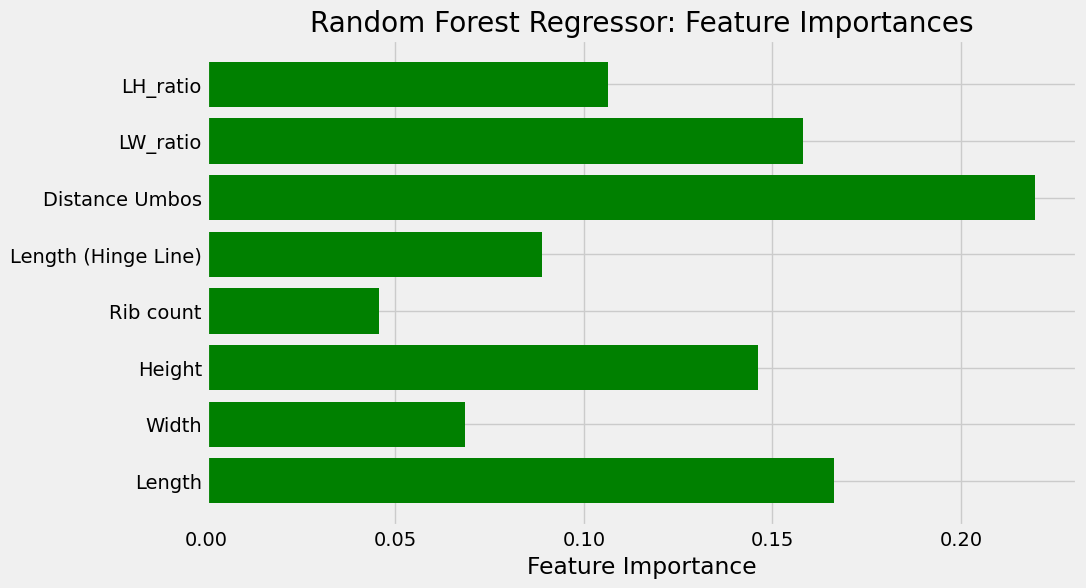
\includegraphics[width=0.8\textwidth]{figures/random-forest.png}
	\caption{Feature Importance of Random Forest}
	\label{fig:random-forest}
\end{figure}

To determine the important features that contribute to the classification of sex in \textit{T. granosa}, two machine learning models, decision trees, and random forest were compared based on the importance of the features. The results in figures ~\ref{fig:decision-trees} and ~\ref{fig:random-forest} indicates variations in feature importance between two models, however certain features such as distance of the umbos, LW\_ratio, length, and height consistently emerge as influential predictors. Hence, this analysis allowed the researchers to identify which features were most predictive that can improve the model’s performance. 

